%Note di Ingegneria del Software
%Sommario: Economicità, Genesi dei processi, standards

\cornell{Economicità}{Principio base del lavoro\\
Riassumibile come l'insieme di efficienza ed efficacia.}

\cornell{Nascita dei processi}{I processi sono nati dai committenti insoddisfatti del lavoro dei fornitori.\\
Sono nate iniziative per vincolare i fornitori a certe regole.\\
Noi ci occuperemo di uno standard generale (esistono anche standard settoriali).\\
Prime applicazioni dei processi: USA (dipartimento della difesa)}

\cornell{Visioni}{Uno standard può essere visto in due modi \begin{itemize}
\item Riferimento a cui vorremmo aderire (best practice)
\item Riferimento a cui dobbiamo assolutamente aderire (Standard imposto) $\Longrightarrow$ Modello di azione (opposto a "modello di valutazione")
\end{itemize}\\
A volte uno standard può essere sia un modello d'azione che un modello di valutazione.}

\cornell{Standard ISO/IEC 12207:1995}{Generato dall'unione di più standard (soprattutto del Dipartimento della Difesa).\\
È uno standard \textbf{astratto}, parla dei processi da usare laddove esiste un ciclo di vita.\\
Esistono 3 macroclassi di processi \begin{description}
\item [Processi Primari] Esistono necessariamente laddove esiste un progetto
\item [Processi Organizzativi] A supporto del lavoro collettivo. Anche attraverso più progetti. Devono esistere affinchè l'organizzazione sia produttiva
\item [Processi di Supporto] Aiutano i processi primari ed organizzativi
\end{description}}

\cornell{Processi Primari}{\begin{itemize}
\item Acquisizione
\item Fornitura
\item Sviluppo
\item Uso/Operazione
\item Manutenzione
\end{itemize}\\
Noi ci occuperemo dei primi 3.}

\cornell{Processi di Supporto}{\begin{itemize}
\item Documentazione
\item Gestione della configurazione
\item Verifica (Tramite misurazioni)
\item Validazione
\item \ldots
\end{itemize}}

\cornell{Processi Organizzativi}{\begin{itemize}
\item Gestione (Qui finiscono e si fanno le misurazioni così da mantenere affidabilità e non invasività)
\item Training/Formazione
\item \ldots
\end{itemize}}

\cornell{Modifica Dello Standard}{Nel 2008 lo standard 12207 è stato esteso dato che il software è divenuto sempre più diffuso, fino ad arrivare a controllare sistemi al di fuori dei computer. Quindi si è aggiunto parte dello standard di qualità riguardante i sistemi.}

\cornell{Sistema}{Aggregato di cose (hardware, software e persone) che hanno un'unico fine comune}

\cornell{Flusso Decisionale}{Governato dall'organizzazione, istanziato in un progetto che a sua volta fa uso dell'engineering.}

\cornell{Organizzazione}{Vi sono solitamente tanti settori dell'azienda, ognuno col suo modo di lavorare.\\
Il compito dell'organizzazione è prendere uno standard generico ed adattarlo alla propria azienda.\\
Un progetto, a sua volta, prende i processi aziendali e li istanzia in sè, nella forma di processi di progetto.\\
Questo processo è detto specializzazione di processi.\\
L'organizzazione interna dei processi dovrebbe essere incentrata sul principi di miglioramente continuo.}

\cornell{Miglioramento Continuo}{\begin{itemize}
\item Pianifico
\item Eseguo secondo i piani
\item Valuto l'esito delle azioni di miglioramento
\item Agisco standardizzando ciò che è andato bene e correggendo le carenze.
\end{itemize}
Questo viene fatto ciclicamente.\\
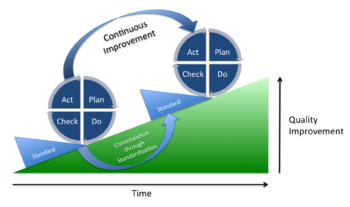
\includegraphics[scale=0.7]{images/2.png}\\
Lo standard funge da "cuneo", impedendo di peggiorare, mentre il miglioramento continua a spingere più in là la qualità. La standardizzazione "sposta" il cuneo verso un nuovo punto massimo.
}
